\section{Durchführung}
\label{sec:Durchführung}

\subsection{Justierung}
Als erstes muss der Aufbau richtig ausgerichtet werden. Dazu wird ein Justierlaser verwendet, der auf der optischen Schiene steht. Zunächst wird das ebenfalls auf der Schiene stehende Plasmarohr ausgerichtet, indem die Justierschrauben so verstellt werden, dass das Licht des Justierlasers das Fadenkreuz am Ende der optischen Schiene trifft.
Anschließend wird ein Resonatorspiegel aufgestellt. Mit den Justierschrauben wird dieser ebenfalls so ausgerichtet, dass der Laser das Fadenkreuz auf der anderen Seite trifft. Mit dem zweiten Resonatorspiegel wird genauso verfahren. Der Justierlaser wird anschließend ausgeschaltet. Der Aufbau ist in \ref{fig:aufbau} zu sehen.

\begin{figure}
    \centering
    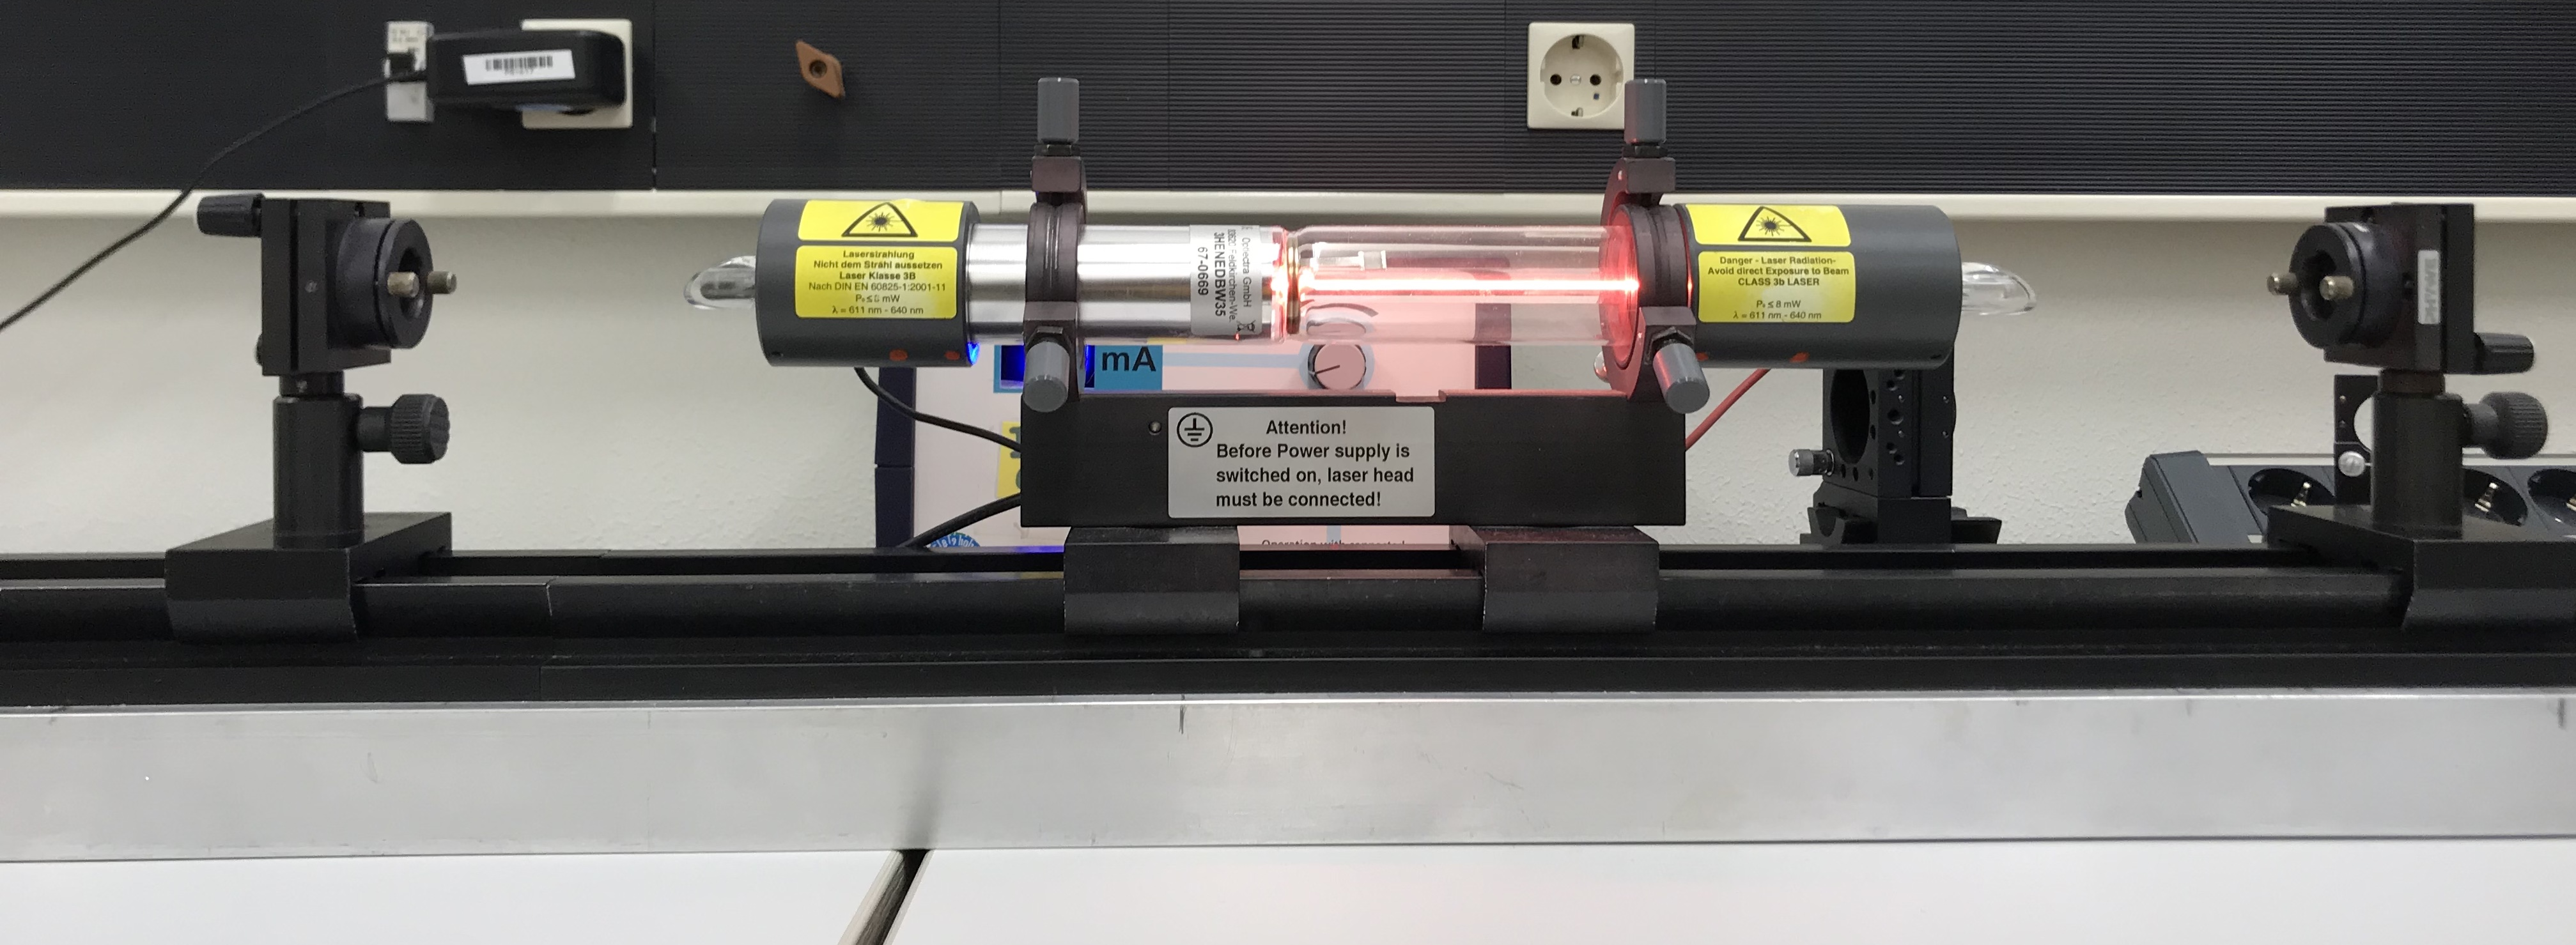
\includegraphics[width=12cm]{fotos/Aufbau2.JPG}
    \caption{Der Versuchsaufbau: Laserrohr und Resonatorspiegel auf der optischen Schiene.}
    \label{fig:aufbau}
\end{figure}    


\subsection{Überprüfung der Stabilitätsbedingung}
Der Strom der Hochspannung wird auf $I = \SI{6.5}{\milli\ampere}$ eingestellt, wodurch das Laserrohr rot leuchtet. Damit die Lasertätigkeit einsetzt, müssen die Resonatorspiegel nachjustiert werden.

Sobald der Laser läuft, wird er mithilfe einer Photodiode auf maximale Leistung eingestellt.
Der Resonatorabstand wird vergrößert und dabei die Leistung aufgenommen. Dabei müssen jedes mal die Spiegel nachjustiert werden, sodass die Leistung maximal ist. 
Der maximale Abstand der Resonatoren soll eingestellt werden.
Diese Messung wird für einen weiteren Resonator erneut durchgeführt.


\subsection{Vermessung von TEM-Moden}
Es werden verschiedene Moden vermessen. Zunächst wird die TEM$_{00}-$Mode vermessen. Dazu wird der Strahldurchmesser mit einer Streulinse vergrößert. Mit einer Photodiode wird die Intensitätsverteilung senkrecht zur Strahlachse gemessen.

Anschließend wird ein Draht aus Wolfram zwischen Resonatorspiegel und Laserrohr gestellt, der dafür sorgt, dass die TEM$_{01}$-Mode und TEM$_{02}$-Mode sichtbar werden. Die Intensitätsverteilungen dieser Moden werden ebenfalls vermessen.


\subsection{Messung der Polarisation}
Die Polarisation des Lasers wird mit einem Polarisator und einer Photodiode, die die Intensität für verschiedene Polarisationen bestimmt, gemessen.
Der Polarisator wird dafür hinter den Auskoppelspiegel gestellt und es werden verschiedene Winkel eingestellt.


\subsection{Bestimmung der Wellenlänge}
Zuletzt wird die Wellenlänge des He-Ne-Lasers bestimmt, indem drei verschiedene Gitter in den Aufbau gesetzt werden und der Abstand der Beugungsmaxima des entstehenden Beugungsbildes vermessen wird.